\documentclass[]{article}
\usepackage{lmodern}
\usepackage[a4paper, total={6in, 8in}]{geometry}
\usepackage{geometry}
\geometry{
	a4paper,
	total={210mm,297mm},
	left=20mm,
	right=20mm,
	top=20mm,
	bottom=20mm,
}
\usepackage{listings}
\usepackage{graphicx}
\usepackage{ifxetex,ifluatex}
\usepackage{fixltx2e} % provides \textsubscript
\ifnum 0\ifxetex 1\fi\ifluatex 1\fi=0 % if pdftex
  \usepackage[T1]{fontenc}
  \usepackage[utf8]{inputenc}
\else % if luatex or xelatex
  \ifxetex
    \usepackage{mathspec}
    \usepackage{xltxtra,xunicode}
  \else
    \usepackage{fontspec}
  \fi
  \defaultfontfeatures{Mapping=tex-text,Scale=MatchLowercase}
  \newcommand{\euro}{€}
\fi
% use upquote if available, for straight quotes in verbatim environments
\IfFileExists{upquote.sty}{\usepackage{upquote}}{}
% use microtype if available
\IfFileExists{microtype.sty}{%
\usepackage{microtype}
\UseMicrotypeSet[protrusion]{basicmath} % disable protrusion for tt fonts
}{}
\ifxetex
  \usepackage[setpagesize=false, % page size defined by xetex
              unicode=false, % unicode breaks when used with xetex
              xetex]{hyperref}
\else
  \usepackage[unicode=true]{hyperref}
\fi
\hypersetup{breaklinks=true,
            bookmarks=true,
            pdfauthor={},
            pdftitle={},
            colorlinks=true,
            citecolor=blue,
            urlcolor=blue,
            linkcolor=magenta,
            pdfborder={0 0 0}}
\urlstyle{same}  % don't use monospace font for urls
\setlength{\parindent}{0pt}
\setlength{\parskip}{6pt plus 2pt minus 1pt}
\setlength{\emergencystretch}{3em}  % prevent overfull lines
\providecommand{\tightlist}{%
  \setlength{\itemsep}{0pt}\setlength{\parskip}{0pt}}
\setcounter{secnumdepth}{0}

\date{}

% Redefines (sub)paragraphs to behave more like sections
\ifx\paragraph\undefined\else
\let\oldparagraph\paragraph
\renewcommand{\paragraph}[1]{\oldparagraph{#1}\mbox{}}
\fi
\ifx\subparagraph\undefined\else
\let\oldsubparagraph\subparagraph
\renewcommand{\subparagraph}[1]{\oldsubparagraph{#1}\mbox{}}
\fi
\title {Marker based localization \\ [10pt]
	Watershed Segmentation  \\[25pt] Team members }
\author {Niharika Jayanthi \and Dheeraj Kamath}
\begin{document}
\maketitle
\begin{center}
	\begin{large}
		Under the guidance of\\
		\textbf{Sanam Shakya}\\
		\vspace{0.5in}
	\end{large}
\end{center}
\section{Goal}\label{goal}

\emph{\textbf{\large In this chapter,}} 
\begin{itemize} 
	\Large
	\item How to use marker-based water shed segmentation on images.
    \item  We will see: \textbf{cv2.distanceTransform()}, \textbf{cv2.watershed()}
\end{itemize}

\section{Theory}\label{theory}
\Large
Watershed is an algorithm in image processing used for isolating objects in the image from the background. The algorithm accepts a grayscale image and a marker image. The markers is an image where you tell the watershed about the foreground objects and the background. \\
\\
\Large{\textbf{Working principle}} \\
Any grayscale image can be viewed as a topographic surface where high intensity denotes peaks and hill while low intensity denotes valleys. We start filling every isolated valleys( local minima) with different colored water. As water rises , depending on the peaks (gradients) nearby, water from different valleys, labeled with different colors will start to merge. To prevent this barriers are built in the locations where the water merges. We continue doing this till all peaks under water. The result will be a segmentation of the image. But this method gives a over segmented image due to noise or any other irregularities in the image. So a major enhancement in the water shed transformation consists in flooding the topographic surface from previously defined set of markers. It is an interactive image segmentation.
What we do is to give different labels for our object we know. Label the region which we are sure of being the foreground or object with one color (or intensity), label the region which we are sure of being background or non-object with another color and finally the region which we are not sure of anything, label it with 0. That is our marker. Then apply watershed algorithm. Then our marker will be updated with the labels we gave, and the boundaries of objects will have a value of -1.

\section{Applications}\label{additional-resources}

\begin{enumerate}
	\item Watershed algorithm is used to monitor traffic. It automatically segments the lanes of a road to count the number of vehicles on different lanes.
	\item It can be used to detect fractures in the surface of steel.
	\item Counting of objects in images can be done using watershed algorithm. An example is counting of coffee beans.
\end{enumerate}
\newpage
\section{Code}\label{code}

1) Since segmentation needs an image in grayscale, we use the following code to convert the image to grayscale.

\begin{verbatim}
'''
*********************************************************************
*                                                                   *
*          IMAGE PROCESSING ( WATERSHED SEGMENTATION )              *
*                                                                   *
*                                                                   *
*  TEAM MEMBERS : NIHARIKA JAYANTHI, DHEERAJ KAMATH                 *
*                                                                   *
*  MENTOR : SANAM SHAKYA                                            *
*                                                                   *
*  FILENAME : watershed.py                                         *
*                                                                   *
*  THEME : DEVELOP MODULES FOR IMAGE PROCESSING AND                 *
*          ROBOT LOCALISATION USING MARKERS                         *
*                                                                   *
*  FUNCTIONS : cv2.watershed(), cv2.distanceTransform()             *
*                                                                   *
*  GLOBAL VARIABLES : NONE                                          *
*                                                                   *
*********************************************************************
'''
\end{verbatim}



\lstinputlisting[language=Python]{watershed.py}

\newpage
Output Images:

\begin{enumerate}
\def\labelenumi{\arabic{enumi})}
\item Input Image\\
   \begin{figure}[h]
   	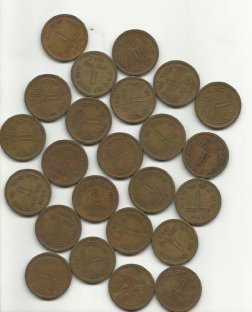
\includegraphics{watercoins.jpg}
   \end{figure}
\newpage
\item Otsu thresholding output image\\
\begin{figure}[h]
	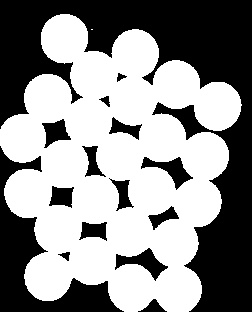
\includegraphics{otsuthresh.jpg}
\end{figure}
\newpage
\item Sure background output image\\
  \begin{figure}[h]
  	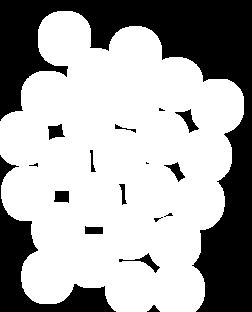
\includegraphics{Surebg.jpg}
  \end{figure}
\newpage
\item Sure foreground output image\\
  \begin{figure}[h]
	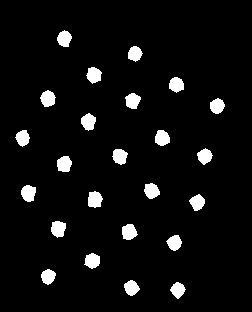
\includegraphics{Surefg.jpg}
  \end{figure}

\newpage   
\item
  Final output image\\
  \begin{figure}[h]
  	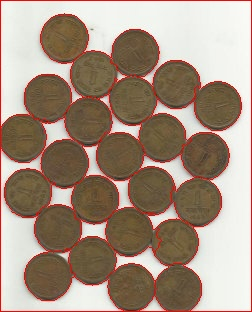
\includegraphics{img.jpg}
  \end{figure}
  
\end{enumerate}
\newpage
\section{Additional Resources}\label{additional-resources}

\begin{enumerate}
\def\labelenumi{\arabic{enumi})}
\tightlist
\item \url{http://cmm.ensmp.fr/~beucher/wtshed.html\#examples}
\item \href{http://opencv-python-tutroals.readthedocs.org/en/latest/py
\_tutorials/py\_imgproc/py\_watershed/py\_watershed.html\#watershed}{About watershed segmentation}
\item \href{https://www.cs.auckland.ac.nz/courses/compsci773s1c/lectures
/ImageProcessing-html/topic3.htm}{Image processing lectures}
\item \href{http://stackoverflow.com/questions/11294859 \\ /how-to-define-the-markers-for-watershed-in-opencv}{Info on defining markers}
\end{enumerate}



\end{document}
